\section{Model Description}
\label{sec:model_010}

We consider a sequence $[e_1,\ldots, e_n]$ of events $\Event_\IndexEvent = (\Class_\IndexEvent, \Timestamp_\IndexEvent)$, where $\Class_\IndexEvent\in \{1,\ldots,\NbClasses\}$ denotes the class of the $\IndexEvent$th event and $\Timestamp_\IndexEvent\in \mathbb{R}$ is its time of occurrence. We assume the events arrive over time, i.e.\ $t_{\IndexEvent}>t_{\IndexEvent-1}$, and we introduce $\DeltaTime^*_\IndexEvent = \Timestamp_\IndexEvent - \Timestamp_{\IndexEvent-1}$ as the observed time gap between the $\IndexEvent$th and the $(\IndexEvent-1)$th event. The history preceding the $\IndexEvent$th event is denoted by $\History_{\IndexEvent}$.
Let $\Simplex=\{\bm{p} \in [0,1]^\NbClasses, \sum_\IndexClass p_\IndexClass = 1\}$ denote the set of probability vectors that form the $(\NbClasses-1)$-dimensional simplex, and $P(\theta)$ be a family of probability distributions on this simplex parametrized by parameters $\theta$. Every sample $\bm p \sim P(\theta)$ corresponds to a (categorical) class distribution.

Given $\Event_{\IndexEvent-1}$ and $\History_{\IndexEvent-1}$, our goal is to model the evolution of the class probabilities, and their uncertainty, of the next event $\IndexEvent$ over time. Technically, we model parameters $\theta(\DeltaTime)$, leading to a distribution $P$ over the class probabilities $\bm p$ for all $\DeltaTime \geq 0$. Thus, we can estimate the most likely class after a time gap $\DeltaTime$ by calculating $\arg\!\max_c \bm{\bar p}(\DeltaTime)_c$, where $\smash{\bm{\bar p}(\DeltaTime) := \E_{\bm p(\DeltaTime) \sim P(\theta(\DeltaTime))}[\bm p(\DeltaTime)]}$ is the expected probability vector. Even more, since we do not consider a point estimate, we can get the amount of certainty in a prediction. For this, we estimate the probability of class $\IndexClass$ being more likely than the other classes, given by $\smash{q_\IndexClass(\DeltaTime) := \E_{\bm p(\DeltaTime) \sim P(\theta(\DeltaTime))}[\mathbb{1}_{\bm p(\DeltaTime)_\IndexClass \geq  \max_{c'\neq c} \bm p(\DeltaTime)_{c'}}]}$. This tells us how certain we are that one class is the most probable (i.e.\ 'how often' is $c$ the argmax when sampling from $P$).

Two expressive and well-established choices for the family $P$ are the Dirichlet distribution and the logistic-normal distribution (app.\ref{distributions}). Based on a common modeling idea, we present two models that exploit the specificities of these distributions: the \GPModel (\cref{GP}) and the \DirModel (\cref{dirichlet}). We also introduce a novel loss to train these models in \cref{uncertainty_loss}.

Independent of the chosen model, we have to tackle two core challenges: (1) \textbf{Expressiveness.} Since the time dependence of $\theta(\DeltaTime)$ may be of different forms, we need to capture complex behavior. (2) \textbf{Locality.} For regions out of the observed data we want to have a higher uncertainty in our predictions. Specifically for $\DeltaTime \rightarrow \infty$, i.e.\  far into the future, the distribution should have a high uncertainty.


\subsection{Logistic-Normal via a Weighted Gaussian Process (\GPModel)}
\label{GP}

\begin{figure}
	\centering
	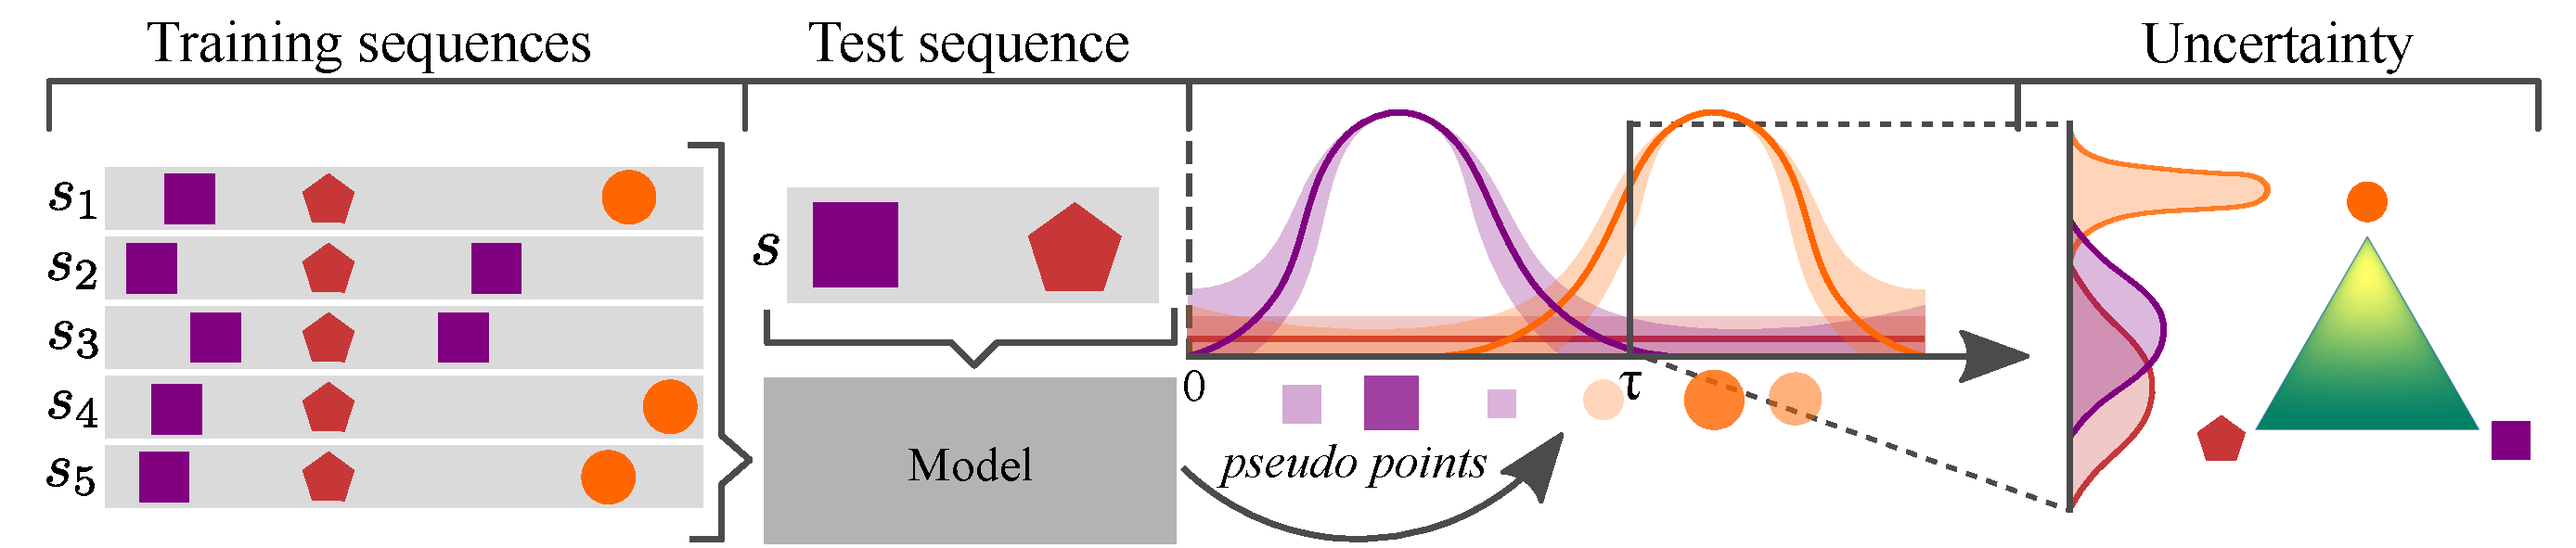
\includegraphics[width=\linewidth]{sections/010_neurips2019/paper/images/model_schema.pdf}
	\begin{subfigure}{0.3\textwidth}
		\caption{} \label{fig:model_illustration_1}
	\end{subfigure}
	\begin{subfigure}{0.69\textwidth}
		\caption{} \label{fig:model_illustration_2}
	\end{subfigure}
	\vspace*{-0.5cm}
    \caption{The model framework. (a) During training we use sequences $s_i$. (b) Given a new sequence of events $s$ the model generates pseudo points that describe $\bm{\theta}(\DeltaTime)$, i.e. the temporal evolution of the distribution on the simplex. These pseudo points are based on the data that was observed in the training examples and weighted accordingly. We also have a measure of certainty in our prediction.}\label{fig:model_illustration}
    \vspace*{-0.5cm}
\end{figure}

We start by describing our model for the case when $P$ is the family of logistic-normal (LN) distributions.
How to model a compact yet expressive evolution of the LN distribution?
Our core idea is to exploit the fact that the LN distribution corresponds to a multivariate random variable whose \textit{logits} follow a \textit{normal distribution} -- and a natural way to model the evolution of a normal distribution is a \textit{Gaussian Process}. Given this insight, the core idea of our model is illustrated in Fig. \ref{fig:model_illustration}: (1) we generate $\NbPoints$ pseudo points based on a hidden state of an RNN whose input is a sequence, (2) we fit a Gaussian Process to the pseudo points, thus capturing the temporal evolution, and (3) we use the learned GP for estimating the parameters $\bm \mu(\DeltaTime)$ and $\bm \Sigma(\DeltaTime)$ of the final LN distribution at any specific time $\tau$. Thus, by generating a small number of points we characterize the full distribution.

\paragraph{Classic GP.}  To keep the complexity low, we train one GP per class $\IndexClass$. That is, our model generates $\NbPoints$ points $(\DeltaTime_\IndexPoint^{(\IndexClass)}, y_\IndexPoint^{(\IndexClass)})$ per class $\IndexClass$, where $y_\IndexPoint^{(\IndexClass)}$ represents logits. Note that the first coordinate of each pseudo point corresponds to time, leading to the temporal evolution when fitting the GP. Essentially we perform a non-parameteric regression from the time domain to the logit space. Indeed, using a classic GP along with the pseudo points, the parameters $\theta$ of the logistic-normal distribution, $\bm \mu$ and $\bm \Sigma$, can be easily computed for any time $\tau$ in closed form:
\begin{equation}\label{eq:gp_prediction}
\begin{aligned}
\mu_{\IndexClass}(\DeltaTime) = \bm{k}_{\IndexClass}^T \bm{K}_{\IndexClass}^{-1} \bm{y}_{\IndexClass},\
\sigma_{\IndexClass}^2(\DeltaTime) = s_{\IndexClass} - \bm{k}_{\IndexClass}^T \bm{K}_{\IndexClass}^{-1} \bm{k}_{\IndexClass}
\end{aligned}
\end{equation}
where  $\bm K_c$ is the  gram matrix w.r.t.\ the $M$ pseudo points of class $c$ based on a  kernel $k$ (e.g. $\smash{k(\DeltaTime_1, \DeltaTime_2) = \exp( -\gamma^2 (\DeltaTime_1 - \DeltaTime_2)^2)}$). Vector $\bm{k}_{\IndexClass}$ contains at position $j$ the value $\smash{k(\DeltaTime_\IndexPoint^{(\IndexClass)},\tau)}$, and $\bm{y}_{\IndexClass}$ the value $\smash{y_\IndexPoint^{(\IndexClass)}}$, and $s_{\IndexClass}=k(\DeltaTime, \DeltaTime)$. At every time point $\DeltaTime$ the logits then follow a multivariate normal distribution with mean $\bm \mu(\DeltaTime)$ and covariance $\smash{\bm \Sigma = \text{diag}(\bm \sigma^2(\DeltaTime))}$.

Using a GP enables us to describe complex functions. Furthermore, since a GP models uncertainty in the prediction depending on the pseudo points, uncertainty is higher in areas far away from the pseudo points. Specifically, it holds for distant future; thus, matching the idea of locality.
%
However, uncertainty is always low around the $M$ pseudo points. Thus $\NbPoints$ should be carefully picked since there is a trade-off between having high certainty at (too) many time points and the ability to capture complex behavior. Thus, in the following we present an extended version solving this problem.

%\begin{wrapfigure}{r}{7cm}
\begin{figure}
	%\vspace*{-0.5cm}
    \centering
    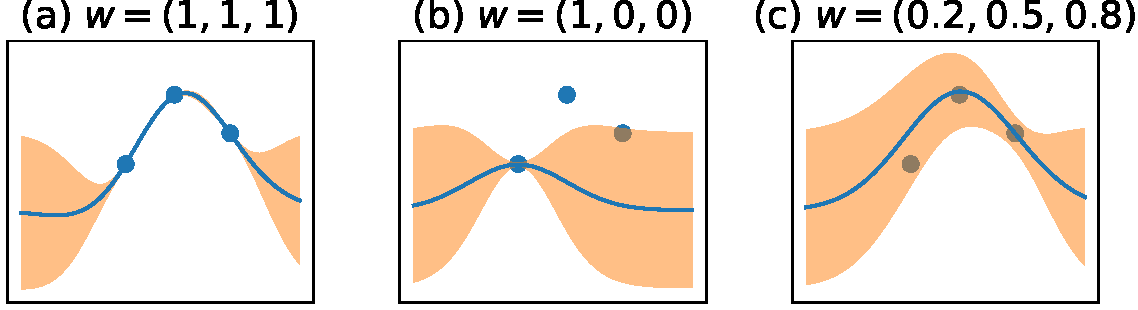
\includegraphics[width=0.8\linewidth]{sections/010_neurips2019/paper/images/weighted_gaussian_process.pdf}
	\caption{WGP on toy data with different weights. (a) All weights are 1 -- classic GP. (b) Zero weights discard points. (c) Mixed weight assignment.}
	\label{fig:weighted_gaussian_process}
%\vspace*{-0.5cm}
\end{figure}
%\end{wrapfigure}

%%%%% Horizontal %%%%%%
%\begin{figure}[H]
%\centering
%\scalebox{0.9}{\begin{tikzpicture}[
%rectanglenode/.style={rectangle, draw=black!100, very thick, minimum size=10mm},
%roundnode/.style={circle, draw=black!100, very thick, minimum size=10mm},
%nonenode/.style={rectangle, draw=none, minimum size=6mm},
%]
%\tikzset{edge/.style = {->,> = latex'}}
%\node[nonenode] (H)         at (-5.9, 10.25)       {$\History$};
%\node[nonenode] (e)      at (-5.9, 9.75)       {$e$};
%\node[rectanglenode] (RNN)       at (-4.5, 10)       {RNN};
%\node[nonenode] (pi)        at (-3, 9.5)       {$w_\IndexPoint^{(\IndexClass)}$};
%\node[nonenode] (mu)       at (-3, 10)       {$\DeltaTime_\IndexPoint^{(\IndexClass)}$};
%\node[nonenode] (sigma)        at (-3,10.5)       {$y_\IndexPoint^{(\IndexClass)}$};
%\node[nonenode] (alpha)        at (-1.5, 10)       {$\theta(\DeltaTime)$};
%\node[nonenode] (p)        at (0.75, 10)       {$\bm{p}(\DeltaTime) \sim P(\theta(\DeltaTime))$};
%\draw[edge] (H) -> (RNN) {};
%\draw[edge] (e) -> (RNN) {};
%\draw[edge] (RNN) -> (pi) {};
%\draw[edge] (RNN) -> (mu) {};
%\draw[edge] (RNN) -> (sigma) {};
%\draw[edge] (pi) -> (alpha) {};
%\draw[edge] (mu) -> (alpha) {};
%\draw[edge] (sigma) -> (alpha) {};
%\draw[edge] (alpha) -> (p) {};
%\end{tikzpicture}}
%\caption{Model diagram. Both models output pseudo points given history and new event. In \GPModel they generate parameters $\theta(\DeltaTime) = \{\bm \mu (\DeltaTime), \bm \Sigma(\DeltaTime)\}$ that model $P(\theta(\DeltaTime))$ as a logistic-normal distribution. In \DirModel these points generate $\theta(\DeltaTime) = \bm \alpha(\DeltaTime)$ to model $P(\theta(\DeltaTime))$ as a Dirichlet distribution.}
%\label{fig:model_diagram}
%\end{figure}
%%%%% Vertical %%%%%%
% \InsertBoxR{3}{\parbox{0.3\linewidth}{
\begin{wrapfigure}[12]{r}{3.5cm}
    \vspace*{-0.6cm}
    \centering
    \scalebox{.75}{\begin{tikzpicture}[
    rectanglenode/.style={rectangle, draw=black!100, very thick, minimum size=10mm},
    roundnode/.style={circle, draw=black!100, very thick, minimum size=5mm},
    nonenode/.style={rectangle, draw=none, minimum size=6mm},
    ]
    \tikzset{edge/.style = {->,> = latex'}}
    \node[nonenode] (H)         at (8.7,4.5)       {$\History_{\IndexEvent-1}$};
    \node[nonenode] (e)      at (10,5.6)       {$e_{\IndexEvent-1}$};
    \node[rectanglenode] (RNN)       at (10,4.5)       {RNN};
    \node[nonenode] (pi)        at (9.25,3.4)       {$[w_\IndexPoint^{(\IndexClass)},$};
    \node[nonenode] (mu)       at (10,3.4)       {$\DeltaTime_\IndexPoint^{(\IndexClass)},$};
    \node[nonenode] (sigma)        at (11,3.4)       {$y_\IndexPoint^{(\IndexClass)}]_{\IndexPoint=1}^\NbPoints$};
    \node[roundnode] (regression)        at (10,2.4)       {GP};
    \node[nonenode] (alpha)        at (10,1.4)       {$\DeltaTime_{\IndexClass}(\DeltaTime), \sigma_{\IndexClass}^2(\DeltaTime)$};
    \node[nonenode] (p)        at (10,0.5)       {$\bm{p}(\DeltaTime) \sim P(\theta(\DeltaTime))$};
    \draw[edge] (H) -> (RNN) {};
    \draw[edge] (e) -> (RNN) {};
    \draw[edge] (RNN) -> (pi) {};
    \draw[edge] (RNN) -> (mu) {};
    \draw[edge] (RNN) -> (sigma) {};
    \draw[edge] (pi) -> (regression) {};
    \draw[edge] (mu) -> (regression) {};
    \draw[edge] (sigma) -> (regression) {};
    \draw[edge] (regression) -> (alpha) {};
    \draw[edge] (alpha) -> (p) {};
    \end{tikzpicture}}
    \caption{Model diagram}\label{fig:model_diagram}
% }}[6]
    \vspace*{-1cm}
\end{wrapfigure}

\paragraph{Weighted GP.} We would like to pick $\NbPoints$ large enough to express rich multimodal functions and allow the model to discard unnecessary points.
To do this we generate an additional weight vector $\smash{\bm{w}^{(\IndexClass)} \in [0,1]^\NbPoints}$ that assigns the weight $\smash{w_\IndexPoint^{(\IndexClass)}}$ to a point $\smash{\DeltaTime^{(\IndexClass)}_\IndexPoint}$. Giving a zero weight to a point should discard it, and giving $1$ will return the same result as with a classic GP. To achieve this goal, we introduce a new kernel function:
\begin{equation}
\begin{aligned}\label{eq:weighted_kernel}
    k'(\DeltaTime_1, \DeltaTime_2) &= f(w_1, w_2) k(\DeltaTime_1, \DeltaTime_2)
\end{aligned}
\end{equation}
%\parskip 0pt
where $k$ is the same as above. The function $f$ weights the kernel $k$ according to the weigths for $\DeltaTime_1$ and $\DeltaTime_2$.
We require $f$ to have the following properties: (1) $f$ should be a valid kernel over the weights, since then the function $k'$ is a valid kernel as well; (2) the importance of pseudo points should not increase, giving $f(w_1, w_2) \leq \min(w_1,w_2)$; this fact implies that a point with zero weight will be discarded since $f(w_1, 0)=0$ as desired. The function $f(w_1,w_2)=\min(w_1,w_2)$  is a simple choice that fulfills these properties.
In Fig. \ref{fig:weighted_gaussian_process}  we show the effect of different weights when fitting of a GP (see Appendix \ref{gp_min_kernel} for a more detailed discussion of the behavior of the $\min$ kernel).
%\parskip 5pt
To predict $\mu$ and $\sigma^2$ for a new time $\DeltaTime$, we can now simply apply Eq. \ref{eq:gp_prediction} based on the new kernel $k'$, where the weight for the \textit{query} point $\DeltaTime$ is $1$.

To summarize: From a hidden state $\smash{h_\IndexEvent = \text{RNN}(\Event_{\IndexEvent-1}, \History_{\IndexEvent-1})}$ we use a a neural network to generate $\NbPoints$ weighted pseudo points $(w_\IndexPoint^{(\IndexClass)}, \DeltaTime_\IndexPoint^{(\IndexClass)}, x_\IndexPoint^{(\IndexClass)})$ per class $\IndexClass$.
Fitting a Weighted GP to these points enables us to model the temporal evolution of $\smash{\mathcal{N}(\mu_\IndexClass(\DeltaTime), \sigma_\IndexClass^2(\DeltaTime))}$ and, thus, accordingly of the logistic-Normal distribution. Fig. \ref{fig:model_diagram} shows an illustration of this model.
%
Note that the cubic complexity of a GP, due to the matrix inversion, is not an issue since the number $\NbPoints$ is usually small ($<10$), while still allowing to represent rich multimodal functions. Crucially, given the loss defined in Sec.\ \ref{uncertainty_loss}, our model is fully differentiable, enabling us efficient training.



\subsection{Dirichlet via a Function Decomposition (\DirModel)}
\label{dirichlet}

Next, we consider the Dirichlet distribution to model the uncertainty in the predictions. The goal is to model the evolution of the concentrations parameters $\bm{\alpha}=(\alpha_1, \dots,\alpha_\NbClasses)^T$ of the Dirichlet over time. 
Since unlike to the logistic-normal, we cannot draw the connection to the GP, we propose  to decompose the parameters of the Dirichlet distribution with expressive (local) functions in order to allow complex dependence on time. 
 %
Since the concentration parameters $\alpha_\IndexClass(\DeltaTime)$  need to be positive, we propose the following decomposition of $\alpha_\IndexClass(\DeltaTime)$ in the log-space
\begin{equation}\label{eq:fct_dec}
\begin{aligned}
\log \alpha_\IndexClass(\DeltaTime) &= \sum_{\IndexPoint=1}^{\NbPoints} w_\IndexPoint^{(\IndexClass)} \cdot \mathcal{N}(\DeltaTime|\DeltaTime_\IndexPoint^{(\IndexClass)}, \sigma_\IndexPoint^{(\IndexClass)}) + \nu
%f(\DeltaTime, \theta_\IndexPoint^{(\IndexClass)}) + \nu
\end{aligned}
\end{equation}

where the real-valued scalar $\nu$ is a constant prior on $\log \alpha_\IndexClass(\DeltaTime)$ which takes over in regions where the Gaussians are close to $0$.

The decomposition into a sum of Gaussians is beneficial for various reasons: 
\textbf{(i)} First note that the concentration parameter $\alpha_\IndexClass$ can be viewed as the effective number of observations of class $\IndexClass$. Accordingly the larger $\log \alpha$, the more certain becomes the prediction. Thus, the functions $\smash{\mathcal{N}(\DeltaTime|\DeltaTime_\IndexPoint^{(\IndexClass)}, \sigma_\IndexPoint^{(\IndexClass)})}$ can describe time regions where we observed data and, thus, should be more certain; i.e. regions around the time $\smash{\DeltaTime_\IndexPoint^{(\IndexClass)}}$ where the 'width' is controlled by $\smash{\sigma_\IndexPoint^{(\IndexClass)}}$.
\textbf{(ii)} Since most of the functions'  mass is centered around their mean, the locality property is fulfilled. Put differently: In regions where we did not observed data (i.e. where the functions $\smash{\mathcal{N}(\DeltaTime|\DeltaTime_\IndexPoint^{(\IndexClass)}, \sigma_\IndexPoint^{(\IndexClass)})}$ are close to $0$), the value $\log \alpha_\IndexClass(\DeltaTime)$ is close to the prior value $\nu$. In the experiments, we use $\nu=0$ , thus $\alpha_\IndexClass(\DeltaTime)=1$ in the out of observed data regions; a common (uninformative) prior value for the Dirichlet parameters. Specifically for $\DeltaTime \rightarrow \infty$ the resulting predictions have a high uncertainty.
\textbf{(iii)} Lastly, a linear combination of translated Gaussians is able to approximate a wide family of functions \cite{ApproximatingWithGaussians}. And similar to the weighted GP, the coefficients $\smash{w_\IndexPoint^{(\IndexClass)}}$ allow discarding unnecessary basis functions.
%Henceforth, we will use Gaussians as basis functions. However, other families of functions can also be good candidates (e.g. Wavelets).

The basis functions parameters $\smash{(w_\IndexPoint^{(\IndexClass)}, \DeltaTime_\IndexPoint^{(\IndexClass)}, \sigma_\IndexPoint^{(\IndexClass)})}$ are the output of the neural network, and can also be interpreted as weighted pseudo points that determine the regression of Dirichlet parameters $\theta(\DeltaTime)$, i.e. $\alpha_\IndexClass(\DeltaTime)$, over time (\cref{fig:model_illustration,fig:model_diagram}). The concentration parameters $\alpha_\IndexClass(\DeltaTime)$ themselves have also a natural interpretation: they can be viewed as the rate of events after time gap~$\DeltaTime$.


%\textbf{Uncertainty with Dirichlet Distribution.} %Classification tasks can be easily modelled with a categorical distribution $\textbf{Cat}(\bm{p})$ where $\bm{p}=(p_1,\dots,p_\NbClasses)^T$ is the class probability vector. 
%Given this model, uncertainty on the categorical distribution may be introduced by assuming that probability vector follows a Dirichlet distribution $\bm{p} \sim \textbf{Dir}(\bm{\alpha})$ where $\bm{\alpha}=(\alpha_1, \dots,\alpha_\NbClasses)^T$ is the concentration parameter vector. The mean and the variance of this distribution are
%\begin{equation}
%\begin{aligned}
%\E[p_\IndexClass] = \frac{\alpha_\IndexClass}{\alpha_0} \text{,}\; \textbf{Var}[p_\IndexClass] = \frac{\alpha_\IndexClass(\alpha_0 - \alpha_\IndexClass)}{\alpha_0^2 (\alpha_0+1)}
%\end{aligned}
%\end{equation}
%where $\alpha_0 = \sum_{\IndexClass=0}^{\NbClasses} \alpha_\IndexClass$. Given observations $\bm{m} = (m_1, \dots,m_\NbClasses)^T$, the Bayesian update of the probability vector distribution is simply $\bm{p} \sim \textbf{Dir}(\bm{\alpha} + \bm{m})$. This formula shows us two things:
%\begin{enumerate*}[label=(\roman*)]
%	\item the concentration parameter $\alpha_\IndexClass$ can be viewed as the effective number of observations of class $\IndexClass$
%	\item the posterior distribution becomes more certain with more observations (even if the classes are equiprobable).
%\end{enumerate*}
%
%In the context of the initial problem of adaptive prediction, a simple solution is to learn a different Dirichlet distribution given different time. Therefore, the model is
%\begin{equation}
%\begin{aligned}
%\bm{p}(\DeltaTime)  \sim \textbf{Dir}(\bm{\alpha}(\DeltaTime))
%\end{aligned}
%\end{equation}
%where $\bm{p}(\DeltaTime) = (p_1(\DeltaTime),\dots, p_\IndexClass(\DeltaTime))^T$ and $\bm{\alpha}(\DeltaTime) = (\alpha_1(\DeltaTime),\dots,\alpha_\IndexClass(\DeltaTime))^T$. The time dependent Dirichlet distribution allows both adaptative predictions and uncertainty on the categorical distribution at time $\DeltaTime$. Note that the concentration parameter $\alpha_\IndexClass(\DeltaTime)$ can be interpreted as the number of observed events of type $\IndexClass$ at time $\DeltaTime$.

%\textbf{Computation of $\alpha$-regularizer.} As stated before, the concentration parameters can be interpreted as pseudocounts of events for each category. In the case of a \DirModel, they represent the rate of events at a given time $\DeltaTime$. While training, the model is likely to overfit and learn very large values of alphas. We propose the following additional loss for the $\IndexEvent$th event that acts as a regularizer:
%\begin{equation}
%\begin{aligned}
%r_\IndexEvent = \Big(\alpha_0(\DeltaTime_\IndexEvent) - \sum_j  \mathbb{1}_{\DeltaTime_j \in [\DeltaTime_\IndexEvent-\frac{w}{2}, \DeltaTime_\IndexEvent+\frac{w}{2}]} \Big)^2
%\end{aligned}
%\end{equation}
%where the summation term counts the total number of events which really occurred in a time window of size $w$ around $\DeltaTime_\IndexEvent$. Hence, the regularizer prevents the predicted pseudocounts of events $\alpha_0(\DeltaTime_\IndexEvent)$ to deviate from the true number of events observed at time $\DeltaTime_\IndexEvent$. Here, the true number of events does not depend on the history which allows beforehand computation during the data preprocessing step.

\subsection{Model Training with the Distributional Uncertainty Loss}
\label{uncertainty_loss}

The core feature of our models is to perform predictions in the future with uncertainty.
The classical cross-entropy loss, however, is not well suited to learn uncertainty on the categorical distribution since it is only based on a single (point estimate) of the class distribution. That is, the standard cross-entropy loss for the $\IndexEvent^{\text{th}}$ event between the true categorical distribution $\bm{p}_{\IndexEvent}^{*}$ and the predicted (mean) categorical distribution $\overline{\bm{p}}_{\IndexEvent}$ is
$\mathcal{L}_{\IndexEvent}^{\text{CE}} = \CrossEntropy[\bm{p}_{\IndexEvent}^*, \overline{\bm{p}}_{\IndexEvent}(\DeltaTime_{\IndexEvent}^*)] = - \sum_\IndexClass p_{\IndexEvent \IndexClass}^* \log \overline{p}_{\IndexEvent \IndexClass}(\DeltaTime_{\IndexEvent}^*)$. Due to the point estimate $\overline{\bm{p}}_{\IndexEvent}(\DeltaTime) = \E_{\bm{p}_{\IndexEvent} \sim P_{\IndexEvent}(\theta(\DeltaTime))}[\bm{p}_{\IndexEvent}]$, the uncertainty on $\bm{p}_{\IndexEvent}$ is completely neglected.


Instead, we propose the \UncertaintyLoss which takes into account uncertainty:
\begin{equation}\label{eq:loss}
\begin{aligned}
\mathcal{L}_{\IndexEvent}^{\text{UCE}} = \E_{\bm{p}_{\IndexEvent} \sim P_{\IndexEvent}(\theta(\DeltaTime_{\IndexEvent}^*))}[\CrossEntropy[\bm{p}_{\IndexEvent}^*, \bm{p}_{\IndexEvent}]] = - \int P_{\IndexEvent}(\theta(\DeltaTime_{\IndexEvent}^*)) \sum_\IndexClass p_{\IndexEvent \IndexClass}^* \log p_{\IndexEvent \IndexClass}
\end{aligned}
\end{equation}
\com{Remark that the \UncertaintyLoss does not
use the compound distribution $\overline{\bm{p}}_{\IndexEvent}(\DeltaTime)$ but considers the expected cross-entropy}. Based on Jensen's inequality, it holds: $0 \leq \mathcal{L}_{\IndexEvent}^{\text{CE}} \leq \mathcal{L}_{\IndexEvent}^{\text{UCE}}
$. Consequently, a low value of the \UncertaintyLoss guarantees a low value for the classic cross entropy loss, while additionally taking the variation in the class probabilities into account. A comparison between the classic cross entropy and the \UncertaintyLoss on a simple classification task \com{and anomaly detection in asynchronous event setting} is presented in Appendix \ref{uncertain_loss_classification}.

In practice the true distribution $\bm{p}_{\IndexEvent}^*$ is often a one hot-encoded representation of the observed class $\IndexClass_{\IndexEvent}$ which simplifies the computations. During training, the models compute $P_{\IndexEvent}(\theta(\DeltaTime))$ and evaluate it at the true time of the next event $\DeltaTime_{\IndexEvent}^*$ given the past event $\Event_{\IndexEvent-1}$ and the history $\History_{\IndexEvent-1}$. The final loss for a sequence of events is simply obtained by summing up the loss for each event
$\mathcal{L}=\sum_\IndexEvent \E_{\bm{p}_{\IndexEvent} \sim P_{\IndexEvent}(\theta(\DeltaTime_{\IndexEvent}^*))}[\CrossEntropy[\bm{p}_{\IndexEvent}^*, \bm{p}_{\IndexEvent}]]$.

\textbf{Fast computation.}  In order to have an efficient computation of the \UncertaintyLoss, we propose closed-form expressions.
\textit{(1) Closed-form loss for Dirichlet.} Given that the observed class $\IndexClass_\IndexEvent$ is one hot-encoded by $\bm{p}_\IndexEvent^*$, the uncertain loss can be computed in closed form for the Dirichlet:
\begin{equation} \label{eq:dir_loss}
\mathcal{L}_\IndexEvent^{\text{UCE}} = \E_{\bm{p}_\IndexEvent(\DeltaTime_\IndexEvent^*) \sim \textbf{Dir}(\bm{\alpha}(\DeltaTime_\IndexEvent^*))}[\log p_{\IndexClass_\IndexEvent}(\DeltaTime_\IndexEvent^*)] = \Psi(\alpha_{\IndexClass_\IndexEvent}(\DeltaTime_\IndexEvent^*)) - \Psi(\alpha_0(\DeltaTime_\IndexEvent^*))
\end{equation}
where $\Psi$ denotes the digamma function and $\alpha_0(\DeltaTime_\IndexEvent^*) = \sum_\IndexClass^\NbClasses \alpha_\IndexClass(\DeltaTime_\IndexEvent^*)$.
\textit{(2) Loss approximation for GP.} For \GPModel, we approximate $ \mathcal{L}_\IndexEvent^{\text{UCE}}$ based on second order series expansion (Appendix \ref{loss_closed_form_proof}):
\small
\begin{equation} \label{eq:gp_loss}
    \mathcal{L}_\IndexEvent^{\text{UCE}}
    \approx \mu_{\IndexClass_\IndexEvent}(\DeltaTime_\IndexEvent^*) - \log \Big( \sum_\IndexClass^\NbClasses \exp(\mu_\IndexClass(\DeltaTime_\IndexEvent^*) + \sigma_\IndexClass^2(\DeltaTime_\IndexEvent^*) / 2) \Big) +
        \frac{\sum_\IndexClass^\NbClasses (\exp(\sigma_\IndexClass^2(\DeltaTime_\IndexEvent^*)) - 1) \exp(2 \mu_\IndexClass(\DeltaTime_\IndexEvent^*) + \sigma_\IndexClass^2(\DeltaTime_\IndexEvent^*))}
        {2 \Big( \sum_\IndexClass^\NbClasses \exp(\mu_\IndexClass(\DeltaTime_\IndexEvent^*) + \sigma_\IndexClass^2(\DeltaTime_\IndexEvent^*) / 2) \Big)^2}
\end{equation}
\normalsize

Note that we can now fully backpropagate through our loss (and through the models as well), enabling to train our methods efficiently with automatic differentiation frameworks and, e.g., gradient descent.

\textbf{Regularization.} While the above loss much better incorporates uncertainty, it is still possible to generate pseudo points with high weight values outside of the observed data regime giving us predictions with high confidence. To eliminate this behaviour we introduce a regularization term $r_\IndexClass$:
\begin{equation}\label{gp_regularization}
r_\IndexClass = \alpha \underbrace{\int_0^T (\mu_\IndexClass(\DeltaTime))^2 \,d\DeltaTime}_{\text{Pushes mean to 0}} +
\beta  \underbrace{\int_0^T (\nu - \sigma_\IndexClass^2(\DeltaTime))^2 \,d\DeltaTime}_{\text{Pushes variance to $\nu$}}
\end{equation}
For the \GPModel, $\mu_\IndexClass(\DeltaTime)$ and $\sigma_\IndexClass(\DeltaTime)$ correspond to the mean and the variance of the class logits which are pushed to prior values of $0$ and $\nu$. For the \DirModel, $\mu_\IndexClass(\DeltaTime)$ and $\sigma_\IndexClass(\DeltaTime)$ correspond to the mean and the variance of the class probabilities where the regularizer on the mean can actually be neglected because of the prior $\nu$ introduced in the function decomposition (Eq. \ref{eq:fct_dec}). In experiments, $\nu$ is set to $1$ for \GPModel and $\smash{\frac{\NbClasses-1}{\NbClasses^2(\NbClasses+1)}}$ for \DirModel which is the variance of the classic Dirichlet prior with concentration parameters equal to $1$. For both models, this regularizer forces high uncertainty on the interval $(0, T)$. In practice, the integrals can be estimated with Monte-Carlo sampling whereas $\alpha$ and $\beta$ are hyperparameters which are tuned on a validation set.

In \citep{PriorNetworks}, to train models capable of uncertain predictions,  another dataset or a generative models to access out of observed distribution samples is required. In contrast, our regularizer suggests a simple way to consider out of distribution data which does not require another model or dataset.


%\subsection{Model Framework}
\label{model_framework}



\
After training is finished we are given a new asynchronous sequence of events. The two models generate $\NbPoints$ pseudo points per class $\IndexClass$ in the future when they expect event of this type. In our case, the pseudo points are denoted by $\smash{\mu_\IndexPoint^{(\IndexClass)}}$ for \DirModel and by $\smash{\DeltaTime_\IndexPoint^{(\IndexClass)}}$ for a \GPModel. Each pseudo point is weighted to express the probability of the occurrence of class $\IndexClass$ and the amount of certainty for this prediction in the surrounding time interval. These values are denoted by $\smash{c_\IndexPoint^{(\IndexClass)}}$ and $\smash{\sigma_\IndexPoint^{(\IndexClass)}}$ for a \DirModel, and by $\smash{w_\IndexPoint^{(\IndexClass)}}$ and $\smash{x_\IndexPoint^{(\IndexClass)}}$ for a \GPModel.

Finally, pseudo points are used to describe the potentially complex evolution of the categorical distribution $\bm{p}_{\IndexEvent+1}(\DeltaTime)$ over time.

%We are modelling this in the logit space by using a function decomposition for \DirModel and a Gaussian process for \GPModel. The logit space is a meaininful choice since the categorical distribution belongs to the exponential family and its natural parameters are logits. By working in the logits space, the natural parameters are not constrained on the interval $[0,1]$.

%One major difference between the two models is where and how the uncertainty is introduced. For \DirModel, only the categorical distribution is uncertain and $\bm{p}_{\IndexEvent+1}(\DeltaTime)$ follows a Dirichlet distribution. In contrast, for \GPModel, both the logits and the categorical distribution are uncertain. The logits follow normal distribution and $\bm{p}_{\IndexEvent+1}(\DeltaTime)$ follows a logit normal distribution.


% !TeX root = ./nips_2019.tex

\section{Point Process Framework} 

%\bc{
%\begin{itemize}
%\item Here, we want to show that with an extension using the point process framework, our models can model the distribution on classes AND time. This was not possible with the first versions of our models. Moreover it allows later to have a closer comparison with our competitors (Neural Hawkes and RMTPP)
%\item The only practical modification is the two new terms (ii) and (iii) in the loss which emerge from the maximization of the likelihood of the joint distribution instead of the conditional distribution.
%\item Conceptually the function decomposition does not learn now $\theta(\tau)$ but intensity parameters of point processes.
%\end{itemize}} \sg{for me it is not clear what we want to say here. do we want to say that our models are more flexible? that they generalize the Point Process framework??? also: are we then USING this point process idea? and what do we then actually change?? do we use eq (13) as a loss? i really don't understand this part!} \sg{or are we essentially saying that we do not model $\theta(\tau)$ as I described it; but rather the intensity function???}

Our models \DirModel and \GPModel predict $P(\theta(\DeltaTime))$, enabling to evaluate, e.g., $\overline{\bm{p}}$ after a specific time gap $\tau$. This corresponds to a conditional distribution $q(\IndexClass|\DeltaTime):=\overline{p}_{\IndexClass}(\DeltaTime)$ over the classes.
In this section, we introduce a \emph{point process} framework to generalize \DirModel to also predict the time distribution $q(\DeltaTime)$. This enables us to predict, e.g., the most likely time the next event is expected or to evaluate the joint distribution $q(c|\tau)\cdot q(\DeltaTime)$. We call the model \DirModel-PP.

We modify the model so that each class $\IndexClass$ is modelled using an inhomogeneous Poisson point process with positive locally integrable intensity function $\lambda_\IndexClass(\DeltaTime)$. Instead of generating parameters $\theta(\DeltaTime)= (\alpha_1 (\DeltaTime),...,\alpha_\NbClasses (\DeltaTime))$ by function decomposition, \DirModel-PP generates intensity parameters over time: $\smash{\log \lambda_\IndexClass(\DeltaTime) = \sum_{\IndexPoint=1}^{\NbPoints} w_\IndexPoint^{(\IndexClass)} \mathcal{N}(\DeltaTime|\DeltaTime_\IndexPoint^{(\IndexClass)}, \sigma_\IndexPoint^{(\IndexClass)}) + \nu}$. The main advantage of such general decomposition is its potential to describe complex multimodal intensity functions contrary to other models like RMTPP \cite{RMTPP} (app.~\ref{non_expressiveness_hawkes_rmtpp}). Since the concentration parameter $\alpha_\IndexClass(\DeltaTime)$ and the intensity parameter $\lambda_\IndexClass(\DeltaTime)$ both relate to the number of events of class $\IndexClass$ around time $\DeltaTime$, it is natural to convert one to the other.

Given this $\NbClasses$-multivariate point process, the probability of the next class given time and the probability of the next event time are
$\smash{q(\IndexClass|\DeltaTime) = \frac{\lambda_{\IndexClass}(\DeltaTime)}{\lambda_0(\DeltaTime)}}$ and $\smash{q(\DeltaTime) = \lambda_0(\DeltaTime) e^{-\int_{0}^{\DeltaTime} \lambda_0(s) ds}}$ where $\smash{\lambda_0(\DeltaTime) = \sum_{\IndexClass=1}^{\NbClasses} \lambda_\IndexClass(\DeltaTime)}$. Since the classes are now modelled via a point proc., the log-likelihood of the event $\Event_\IndexEvent = (\IndexClass_\IndexEvent, \DeltaTime_\IndexEvent^*)$ is:
\begin{equation}\label{eq:pp_loss}
\begin{aligned}
\log q(\IndexClass_\IndexEvent, \DeltaTime_\IndexEvent^*) = \log q(\IndexClass_\IndexEvent| \DeltaTime_\IndexEvent^*) + \log q(\DeltaTime_\IndexEvent^*) = \underbrace{\log  \frac{\lambda_{\IndexClass_\IndexEvent}(\DeltaTime_\IndexEvent^*)}{\lambda_{0}(\DeltaTime_\IndexEvent^*)}}_{(i)} + \underbrace{\log \lambda_{0}(\DeltaTime_\IndexEvent^*)}_{(ii)} - \underbrace{\int_{0}^{\DeltaTime_\IndexEvent^*}\lambda_0(t)dt}_{(iii)}
\end{aligned}
\end{equation}
The terms (ii) and (iii) act like a regularizer on the intensities by penalizing large cumulative intensity $\lambda_0(\DeltaTime)$ on the time interval $[\Timestamp_{\IndexEvent-1}, \Timestamp_\IndexEvent]$ where no events occurred. The term (i) is the standard cross-entropy loss at time $\DeltaTime_\IndexEvent$.  Or equivalently, by modeling the distribution $\textbf{Dir}(\lambda_1(\DeltaTime),..,\lambda_\NbClasses(\DeltaTime))$, we see that term (i) is equal to $\mathcal{L}_{\IndexEvent}^{\text{CE}}$ (see \cref{uncertainty_loss}). Using this insight, we obtain our final \DirModel-PP model: We achieve uncertainty on the class prediction by modeling $\lambda_\IndexClass(\DeltaTime)$ as concentration parameters of a Dirichlet distribution and train the model with the loss of \cref{eq:pp_loss} replacing term (i) by $\mathcal{L}_{\IndexEvent}^{\text{UCE}}$. As it becomes apparent \DirModel-PP differs from \DirModel only in the regularization of the loss function, enabling it to be interpreted as a point process.

